\documentclass[11pt]{article}
\usepackage[utf8]{inputenc}
\usepackage[T1]{fontenc}
\usepackage[spanish]{babel}
\usepackage{amsmath}
\usepackage{booktabs}
\usepackage{graphicx}
\usepackage{float}
\usepackage{geometry}
\geometry{margin=2.5cm}
\setlength{\parskip}{0.65em}
\setlength{\parindent}{0pt}
\title{Informe comparativo de views Black-Litterman}
\author{FinPUC}
\date{}
\begin{document}
\maketitle
\section{Objetivo del contraste}
Este informe compara las cuatro familias de views evaluadas bajo la misma arquitectura de tres horizontes, ventanas móviles y test limpio P4. El foco principal es la dinámica del portafolio, porque esta dimensión determina si una mejora financiera puede implementarse sin inducir rotación, concentración o inestabilidad excesiva en la recomendación.
\section{Resultados de la dinámica del portafolio}
\begin{table}[H]
\centering
\resizebox{\textwidth}{!}{%
\begin{tabular}{lrrrrrrrr}
\toprule
View & Turnover & Turn. >20\% & N efectivo & HHI sector & Peso sector líder & Drift L1 & Overlap top-10 & Top-3 retorno sector \\
\midrule
Desempleo macro & 7.3\% & 0.0\% & 194.32 & 0.157 & 26.7\% & 0.083 & 80.0\% & 65.2\% \\
Momentum general & 34.6\% & 54.4\% & 94.21 & 0.261 & 40.8\% & 0.501 & 36.0\% & 81.6\% \\
Momentum top market-cap 6M & 30.7\% & 37.5\% & 122.88 & 0.208 & 32.3\% & 0.392 & 50.4\% & 71.8\% \\
Momentum top/bottom 1Y & 30.7\% & 37.5\% & 122.88 & 0.208 & 32.3\% & 0.392 & 50.4\% & 71.8\% \\
\bottomrule
\end{tabular}
}
\caption{Comparación agregada de dinámica de portafolio por view.}
\label{tab:comparativo:dinamica}
\end{table}

\begin{figure}[H]
\centering
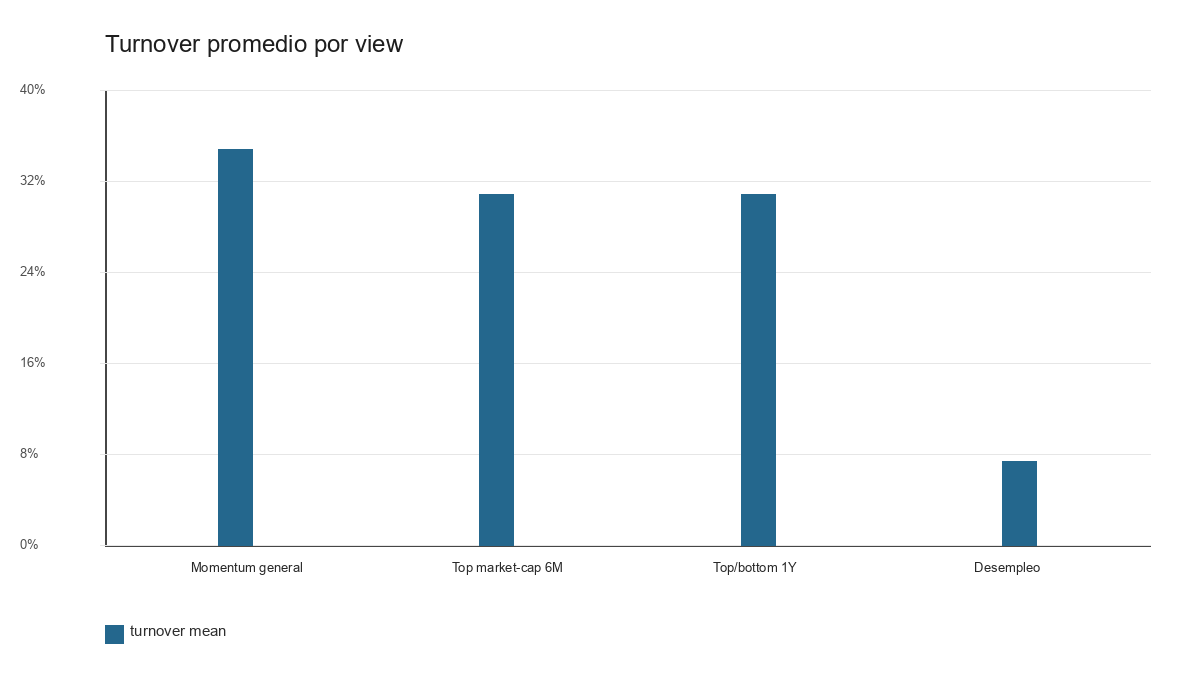
\includegraphics[width=0.86\textwidth]{figuras/comparativo_turnover_views.png}
\caption{Turnover promedio en el horizonte de test limpio por view.}
\label{fig:comparativo:turnover}
\end{figure}
\begin{figure}[H]
\centering
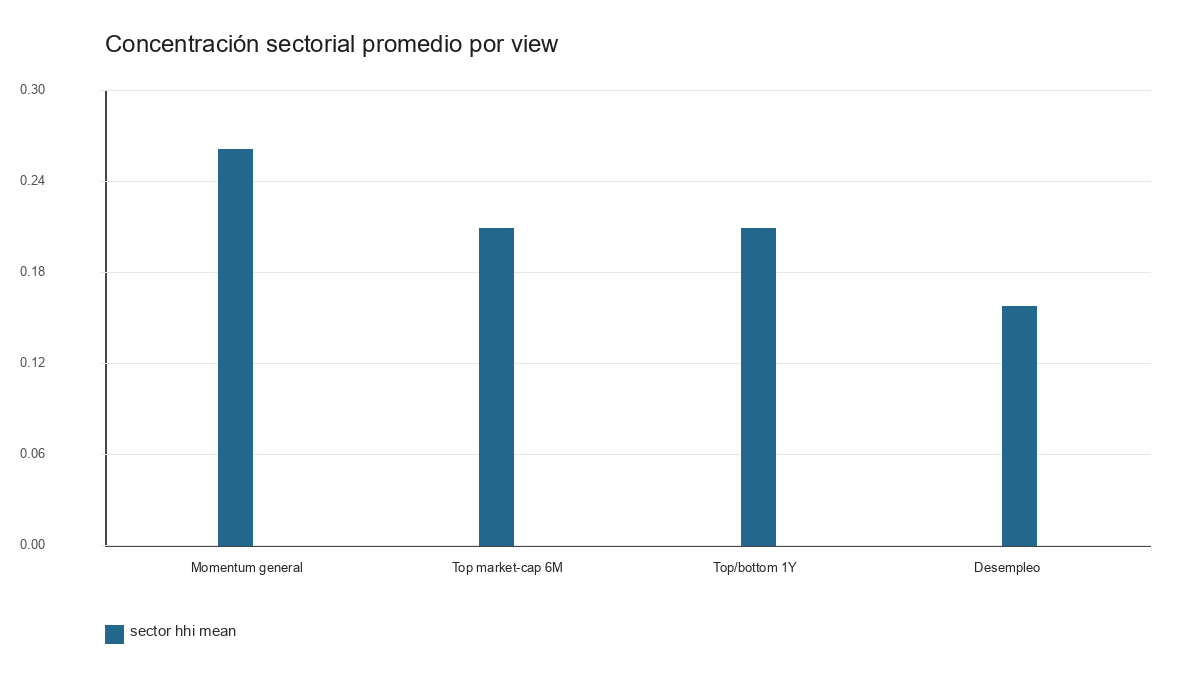
\includegraphics[width=0.86\textwidth]{figuras/comparativo_hhi_sector_views.png}
\caption{Concentración sectorial promedio en el horizonte de test limpio por view.}
\label{fig:comparativo:hhi}
\end{figure}
\begin{figure}[H]
\centering
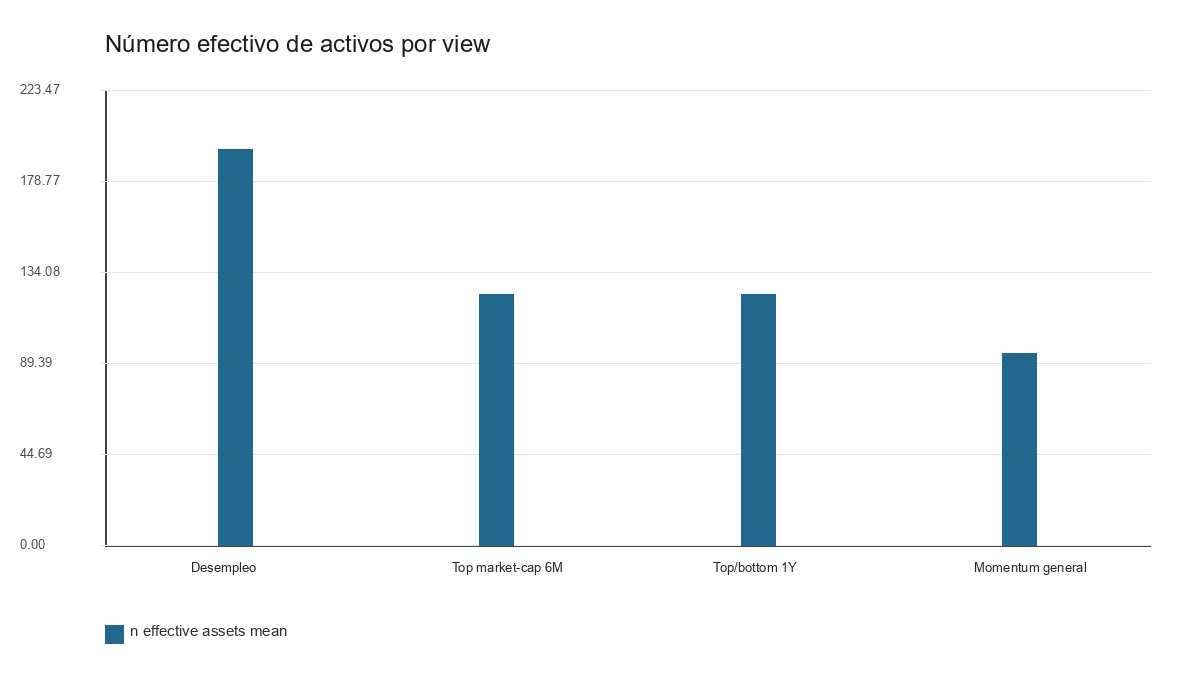
\includegraphics[width=0.86\textwidth]{figuras/comparativo_n_efectivo_views.png}
\caption{Número efectivo de activos promedio en el horizonte de test limpio por view.}
\label{fig:comparativo:neff}
\end{figure}
\section{Lectura financiera y económica}
\begin{table}[H]
\centering
\resizebox{\textwidth}{!}{%
\begin{tabular}{lrrrrrr}
\toprule
View & Mejora Sharpe & \% recomendado & P abandono sem. & Riqueza P4 & Utilidad ex-post & Tasa retiro \\
\midrule
Desempleo macro & 2.0\% & 40.0\% & 100.0\% & 1.004 & 1 & 50.5\% \\
Momentum general & 5.2\% & 40.0\% & 100.0\% & 1.007 & 1 & 54.1\% \\
Momentum top market-cap 6M & -6.1\% & 30.0\% & 100.0\% & 1.005 & 1 & 51.2\% \\
Momentum top/bottom 1Y & -6.1\% & 30.0\% & 100.0\% & 1.005 & 1 & 51.2\% \\
\bottomrule
\end{tabular}
}
\caption{Resumen financiero y económico agregado por view.}
\label{tab:comparativo:p4}
\end{table}

La comparación muestra que la view con mejor estabilidad operacional no necesariamente coincide con la de mayor impulso de Sharpe. En particular, Desempleo macro presenta el menor costo dinámico agregado, mientras que Momentum general entrega la señal financiera promedio más intensa. Esta diferencia es central para la recomendación final: FinPUC no solo debe elegir la mayor rentabilidad esperada, sino una política que pueda sostenerse bajo rebalanceos semestrales y distintos regímenes de mercado.
Un resultado relevante de la calibración es la convergencia empírica entre Momentum top market-cap 6M, Momentum top/bottom 1Y: ambas iteraciones terminan seleccionando la misma estructura congelada de market-cap momentum, por lo que sus métricas de test limpio y dinámica de portafolio coinciden.
\section{Conclusiones generales y recomendaciones}
Como recomendación base para una implementación robusta, Desempleo macro es la view más defendible cuando se prioriza estabilidad, baja rotación y diversificación sectorial. Para perfiles más tolerantes a riesgo, Momentum general puede considerarse una alternativa táctica si el comité acepta el mayor costo dinámico que aparece en la rotación y en la concentración de retornos.
Las views de momentum basadas en market-cap deben presentarse como señales de uso condicionado: su calibración puede identificar estructuras con mejora parcial, pero la dinámica del portafolio revela mayor sensibilidad a cambios de régimen. Por ello, su incorporación final debería limitarse a perfiles que toleren más rebalanceo y exposición sectorial, o bien usarse como módulo complementario y no como recomendación dominante para toda la base de clientes.
\end{document}